\documentclass[11pt]{article}

\usepackage{times}
\usepackage{epsf}
\usepackage{epsfig}
\usepackage{amsmath, alltt, amssymb, xspace}
\usepackage{wrapfig}
\usepackage{fancyhdr}
\usepackage{url}
\usepackage{verbatim}
\usepackage{fancyvrb}

\usepackage{subfigure}
\usepackage{cite}
%\usepackage{cases}
%\usepackage{ltexpprt}
%\usepackage{verbatim}

%\topmargin      -0.70in  % distance to headers
%\headheight     0.2in   % height of header box
%\headsep        0.4in   % distance to top line
%\footskip       0.3in   % distance from bottom line

% Horizontal alignment
\topmargin      -0.50in  % distance to headers
\oddsidemargin  0.0in
\evensidemargin 0.0in
\textwidth      6.5in
\textheight     8.9in 


%\centerfigcaptionstrue

%\def\baselinestretch{0.95}


\newcommand\discuss[1]{\{\textbf{Discuss:} \textit{#1}\}}
%\newcommand\todo[1]{\vspace{0.1in}\{\textbf{Todo:} \textit{#1}\}\vspace{0.1in}}
\newtheorem{problem}{Problem}[section]
%\newtheorem{theorem}{Theorem}
%\newtheorem{fact}{Fact}
\newtheorem{define}{Definition}[section]
%\newtheorem{analysis}{Analysis}
\newcommand\vspacenoindent{\vspace{0.1in} \noindent}

%\newenvironment{proof}{\noindent {\bf Proof}.}{\hspace*{\fill}~\mbox{\rule[0pt]{1.3ex}{1.3ex}}}
%\newcommand\todo[1]{\vspace{0.1in}\{\textbf{Todo:} \textit{#1}\}\vspace{0.1in}}

%\newcommand\reducespace{\vspace{-0.1in}}
% reduce the space between lines
%\def\baselinestretch{0.95}

\newcommand{\fixmefn}[1]{ \footnote{\sf\ \ \fbox{FIXME} #1} }
\newcommand{\todo}[1]{
\vspace{0.1in}
\fbox{\parbox{6in}{TODO: #1}}
\vspace{0.1in}
}

\newcommand{\mybox}[1]{
\vspace{0.2in}
\noindent
\fbox{\parbox{6.5in}{#1}}
\vspace{0.1in}
}


\newcounter{question}
\setcounter{question}{1}

\newcommand{\myquestion} {{\vspace{0.1in} \noindent \bf Question \arabic{question}:} \addtocounter{question}{1} \,}

\newcommand{\myproblem} {{\noindent \bf Problem \arabic{question}:} \addtocounter{question}{1} \,}


\newcommand{\copyrightnoticeA}[1]{
\vspace{0.1in}
\fbox{\parbox{6in}{\small Copyright \copyright\ 2006 - 2014\ \ Wenliang Du, Syracuse University.\\ 
      The development of this document is partially funded by 
      the National Science Foundation's Course, Curriculum, and Laboratory 
      Improvement (CCLI) program under Award No. 0618680 and 0231122. 
      Permission is granted to copy, distribute and/or modify this document
      under the terms of the GNU Free Documentation License, Version 1.2
      or any later version published by the Free Software Foundation.
      A copy of the license can be found at http://www.gnu.org/licenses/fdl.html.}}
\vspace{0.1in}
}


\newcommand{\copyrightnotice}[1]{
\vspace{0.1in}
\fbox{\parbox{6in}{\small Copyright \copyright\ 2006 - 2014\ \ Wenliang Du, Syracuse University.\\
      The development of this document is/was funded by three grants from
      the US National Science Foundation: Awards No. 0231122 and 0618680 from
      TUES/CCLI and  Award No. 1017771 from Trustworthy Computing.
      This lab was imported into the Labtainer framework by the Naval Postgraduate 
      School, Center for Cybersecurity and Cyber Operations under National Science 
      Foundation Award No. 1438893.
      Permission is granted to copy, distribute and/or modify this document
      under the terms of the GNU Free Documentation License, Version 1.2
      or any later version published by the Free Software Foundation.
      A copy of the license can be found at http://www.gnu.org/licenses/fdl.html.}}
\vspace{0.1in}
}

\newcommand{\copyrightnoticeB}[1]{
\vspace{0.1in}
\fbox{\parbox{6in}{\small Copyright \copyright\ 2006 - 2014\ \ Wenliang Du, Syracuse University.\\
      The development of this document is/was funded by the following grants from
      the US National Science Foundation: No. 0231122, 0618680, and 1303306.
      Permission is granted to copy, distribute and/or modify this document
      under the terms of the GNU Free Documentation License, Version 1.2
      or any later version published by the Free Software Foundation.
      A copy of the license can be found at http://www.gnu.org/licenses/fdl.html.}}
\vspace{0.1in}
}


\newcommand{\nocopyrightnotice}[1]{
\vspace{0.1in}
\fbox{\parbox{6in}{\small  
      The development of this document is funded by 
      the National Science Foundation's Course, Curriculum, and Laboratory 
      Improvement (CCLI) program under Award No. 0618680 and 0231122. 
      Permission is granted to copy, distribute and/or modify this document.
      }}
\vspace{0.1in}
}

\newcommand{\idea}[1]{
\vspace{0.1in}
{\sf IDEA:\ \ \fbox{\parbox{5in}{#1}}}
\vspace{0.1in}
}

\newcommand{\questionblock}[1]{
\vspace{0.1in}
\fbox{\parbox{6in}{#1}}
\vspace{0.1in}
}


\newcommand{\minix}{{\tt Minix}\xspace}
\newcommand{\unix}{{\tt Unix}\xspace}
\newcommand{\linux}{{\tt Linux}\xspace}
\newcommand{\ubuntu}{{\tt Ubuntu}\xspace}
\newcommand{\selinux}{{\tt SELinux}\xspace}
\newcommand{\freebsd}{{\tt FreeBSD}\xspace}
\newcommand{\solaris}{{\tt Solaris}\xspace}
\newcommand{\windowsnt}{{\tt Windows NT}\xspace}
\newcommand{\setuid}{{\tt Set-UID}\xspace}
%\newcommand{\smx}{{\tt Smx}\xspace}
\newcommand{\smx}{{\tt Minix}\xspace}
\newcommand{\relay}{{\tt relay}\xspace}
\newcommand{\isys}{{\tt iSYS}\xspace}
\newcommand{\ilan}{{\tt iLAN}\xspace}
\newcommand{\iSYS}{{\tt iSYS}\xspace}
\newcommand{\iLAN}{{\tt iLAN}\xspace}
\newcommand{\iLANs}{{\tt iLAN}s\xspace}
\newcommand{\bochs}{{\tt Bochs}\xspace}

\newcommand\FF{{\mathcal{F}}}

\newcommand{\argmax}[1]{
\begin{minipage}[t]{1.25cm}\parskip-1ex\begin{center}
argmax
#1
\end{center}\end{minipage}
\;
}

\newcommand{\bm}{\boldmath}
\newcommand  {\bx}    {\mbox{\boldmath $x$}}
\newcommand  {\by}    {\mbox{\boldmath $y$}}
\newcommand  {\br}    {\mbox{\boldmath $r$}}


%\pagestyle{fancyplain}
%\lhead[\thepage]{\thesection}      % Note the different brackets!
%\rhead[\thesection]{SEED Laboratories}
%\lfoot[\fancyplain{}{}]{Syracuse University} 
%\cfoot[\fancyplain{}{}]{\thepage} 

\newcommand{\tstamp}{\today}   
%\lhead[\fancyplain{}{\thepage}]         {\fancyplain{}{\rightmark}}
%\chead[\fancyplain{}{}]                 {\fancyplain{}{}}
%\rhead[\fancyplain{}{\rightmark}]       {\fancyplain{}{\thepage}}
%\lfoot[\fancyplain{}{}]                 {\fancyplain{\tstamp}{\tstamp}}
%\cfoot[\fancyplain{\thepage}{}]         {\fancyplain{\thepage}{}}
%\rfoot[\fancyplain{\tstamp} {\tstamp}]  {\fancyplain{}{}}

\pagestyle{fancy}
%\lhead{\bfseries Computer Security Course Project}
\lhead{\bfseries SEED Labs}
\chead{}
\rhead{\small \thepage}
\lfoot{}
\cfoot{}
\rfoot{}

\usepackage{listings}
\usepackage{color}

\definecolor{dkgreen}{rgb}{0,0.6,0}
\definecolor{gray}{rgb}{0.5,0.5,0.5}
\definecolor{mauve}{rgb}{0.58,0,0.82}

\lstset{frame=tb,
  language=C,
  aboveskip=3mm,
  belowskip=3mm,
  showstringspaces=false,
  columns=flexible,
  basicstyle={\small\ttfamily},
  numbers=none,
  numberstyle=\tiny\color{gray},
  keywordstyle=\color{blue},
  commentstyle=\color{dkgreen},
  stringstyle=\color{mauve},
  breaklines=true,
  breakatwhitespace=true,
  tabsize=3
}



\begin{document}

\begin{center}
{\LARGE SSL}
\vspace{0.1in}\\
\end{center}

\copyrightnotice

\section{Overview}
This lab requires that you use SSL certificates to authenticate devices
on a simulated industrial control system network shared by 
Programmable Logic Controlers (PLCs) and Human Machine Inteface (HMI) devices.
The concepts covered by this lab are applicable to pair of clients and servers,
e.g., a web broswer and a web server.

\subsection {Background}
The student is expect to have separately learned about the basic elements of PKI 
certificates, e.g., public/private key pairs, Certification authorities, 
signing requests and certificate chains.  If the student is engaded in independent
study, several tutorial videos that cover public key cryptography are at:
\url{https://my.nps.edu/web/c3o/movies}
Tutorials on the use of the {\tt openssl} utility can be found on the web, and details
can be viewed using ``{\tt man openssl}''.

The student is expected to have at least a basic understanding of the Linux command line,
the basics of the file system, and the ability to use {\tt scp} to copy files from
one computer to another.

\section{Lab Environment}
This lab runs in the Labtainer framework,
available at http://my.nps.edu/web/c3o/labtainers.
That site includes links to a pre-built virtual machine
that has Labtainers installed, however Labtainers can
be run on any Linux host that supports Docker containers.

From your labtainer-student directory start the lab using:
\begin{verbatim}
    labtainer ssl
\end{verbatim}
\noindent A link to this lab manual will be displayed.  

\textbf{All user ids in the lab are {\tt admin} and all passwords are {\tt password}}.

\section{Network Configuration}
This lab includes two sumulated PLCs, two HMI devices, and a certification
authority as shown in Figure~\ref{fig:topology}.
When the lab starts, you will get several virtual terminals, one connected to each
component.

The host names of each component are per the diagram.  The /etc/hosts files
allow use of these host names instead of explicit ip addresses.

Initially, the {\tt plc1} and the {\tt hmi1} components have PKI certificates
and keys provided by the {\tt ca}.  The {\tt hmi1} component includes a 
{\tt client\_ssl} program that sends instructions to a PLC using client-authenticated
TLS.  The {\tt plc1} component includes a {\tt service\_ssl} service that receives
instructions from hmi components.  The SSL connection utilized by the client and server
side of this communication are both authenticated using keys and certificates 
generated using the CA component.

The {\tt plc2} and the {\tt hmi2} components initially lack keys and certificates.  They
include {\tt client} and {\tt server} programs that are functionally identical to those on the
{\tt plc1} and {\tt hmi1} components, except that they do not use SSL.

The ca component is configured for signing certificates within the ``example.com'' domain,
and was used to generated and sign the initial set of certificates.

\begin{figure}[htb]
\begin{center}
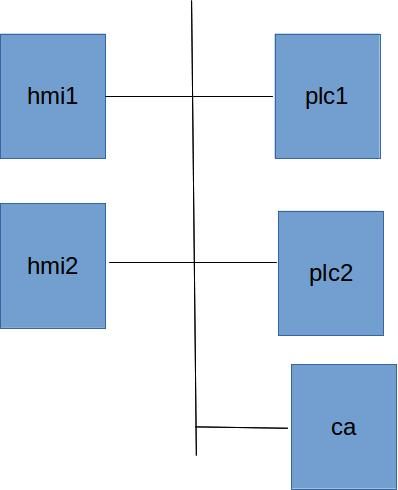
\includegraphics [width=0.8\textwidth,natwidth=621,natheight=403]{ssl.jpg}
\end{center}
\caption{Network topology for the ssl lab}
\label{fig:topology}
\end{figure}

\section{Lab Tasks}
\subsection{Explore}
Start the server\_ssl service on the PLC1 component:
\begin{verbatim}
   ./server_ssl
\end{verbatim}
\noindent and the server service on PLC2:
\begin{verbatim}
   ./server
\end{verbatim}

\noindent Then start wireshark on each of the two HMI components to allow you to
view the network traffic.
\begin{verbatim}
   wireshark &
\end{verbatim}
\noindent Select the {\tt eth0} device.

Then use the client programs on the HMI components to communicate with the PLCs and observe
the network traffic.  On the hm1 component:
\begin{verbatim}
   ./client_ssl plc1 This is an instruction
\end{verbatim}

\noindent and on the hmi2 component:
\begin{verbatim}
   ./client plc2 This is an instruction
\end{verbatim}

What differences do you see in wireshark when you communicate between plc1 and hmi1 as 
opposed to communication between plc2 and hmi2?

Try to send instructions from hmi2 to plc1.  What happens, and why?
Try using the {\tt client\_ssl} program on hmi2 to communicate with each PLC.

Then try to send instructions from hmi1 to plc2.  Again, what happens and why?

\subsection{Generate certficates and keys}
Use the {\tt openssl} utility on the CA component to generate keys and certificates for the {\tt hmi2 and \tt plc2} components.
As an example, the key generation, signing requests and certificate signing operations that were
used for {\tt plc1} are provided below:
\begin{verbatim}
# plc1 key gen
openssl genrsa -out intermediate/private/plc1.example.com.key.pem 2048
chmod 400 intermediate/private/plc1.example.com.key.pem

# plc1 cert signing request
openssl req -config intermediate/openssl.cnf \
      -key intermediate/private/plc1.example.com.key.pem \
      -subj '/CN=plc1.example.com/O=Example./C=US/ST=CA' \
      -new -sha256 -out intermediate/csr/plc1.example.com.csr.pem

# sign plc1 cert
openssl ca -batch -config intermediate/openssl.cnf \
      -extensions server_cert -days 375 -notext -md sha256 \
      -in intermediate/csr/plc1.example.com.csr.pem \
      -out intermediate/certs/plc1.example.com.cert.pem
\end{verbatim}
Before running {\tt openssl} commands, change your directory to the ca directory:
\begin{verbatim}
   cd ~/ca
\end{verbatim}
Generate certificates and keys for plc2, and then for hmi2.  Note when signing 
the hmi2 certificate, you should not include the ``{\tt -extensions server\_cert}'' option
because you are signing a client certificate.

Use scp to transfer files from the CA to the appropriate component.
You will also want to transfer the certificate chain (i.e., the root and intermediate
certificates) from {\tt intermediate/certs/ca-chain.cert.pem} to the {\tt ~/certs} directory 
of the two components.  (Note you have plc1 and hmi1 as working examples).

\subsection{Demonstrate communication between all 4 components}
After installing the certificates and keys, start the {\tt server\_ssl}
service on each of the PLC components.
If you have properly install certificates and keys on hmi2 and plc2, then you should
be able to use the {\tt client\_ssl} program to send instructions to either of the
PLCs from either of the HMI components.  

\section{Submission}
After finishing the lab, go to the terminal on your Linux system that was used to start the lab and type:
\begin{verbatim}
    stoplab 
\end{verbatim}
When you stop the lab, the system will display a path to the zipped lab results on your Linux system.  Provide that file to 
your instructor, e.g., via the Sakai site.

\end{document}
